% !TeX program = lualatex
% !BIB program = biber
% Lualatex is important to render Fira fonts; with pdflatex it's just the regular one
% ratio 16:9 -- https://tex.stackexchange.com/questions/14336/

% compile two versions, inspired by https://tex.stackexchange.com/a/1501
% use the script "compile-pdf.sh"
\newif\ifhandout
% if flags.tex does not exist, create an empty file to be able to compile in TeXstudio
\input{flags}

\ifhandout
	\documentclass[12pt,aspectratio=169,handout]{beamer}
\else
	\documentclass[12pt,aspectratio=169]{beamer}
\fi

% adjust for 16:9
% https://tex.stackexchange.com/questions/354022/modifying-the-margins-of-all-slides-in-beamer
\setbeamersize{text margin left=0.3cm,text margin right=4.5cm} 

%\usepackage{xcolor}

%%% better TOC
\usetheme[subsectionpage=progressbar]{metropolis}

% name in footer
\setbeamertemplate{frame numbering}{\insertframenumber ~ | Dr.\ Ivan Habernal}

% blocks with background globally
\metroset{block=fill}

% adjust the background to be completely white
\setbeamercolor{background canvas}{bg=white}

% typeset mathematics on serif
\usefonttheme[onlymath]{serif}

% better bibliography using biber as backend
\usepackage[natbib=true,backend=biber,style=authoryear-icomp,maxbibnames=30,maxcitenames=9,uniquelist=false,giveninits=true,doi=false,url=false,dashed=false,isbn=false]{biblatex}
% shared bibliography
\addbibresource{../dl4nlp-bibliography.bib}
% disable "ibid" for repeated citations
\boolfalse{citetracker}

\definecolor{76abdf}{RGB}{118, 171, 223}

\setbeamercolor{frametitle}{bg=76abdf, fg=white}

\usepackage{xspace}


% for derivatives, https://tex.stackexchange.com/a/412442
\usepackage{physics}

\usepackage{tikz}
\usetikzlibrary{matrix, positioning}
\usetikzlibrary{angles,quotes} % for angles
\usetikzlibrary{backgrounds} % background
\usetikzlibrary{decorations.pathreplacing} % curly braces
\usetikzlibrary{calligraphy}
\usetikzlibrary{calc} % for neural nets

% for plotting functions
\usepackage{pgfplots}
\usepgfplotslibrary{dateplot}

% sub-figures
\usepackage{caption}
\usepackage{subcaption}

% book tabs
\usepackage{booktabs}


% show TOC at every section start
\AtBeginSection{
	\frame{
		\vspace{2em}
		\sectionpage
		\hspace*{2.2em}\begin{minipage}{10cm}
			\tableofcontents[currentsection]
		\end{minipage}
	}
}

% argmin, argmax
\usepackage{amsmath}
\DeclareMathOperator*{\argmax}{arg\!\max}
\DeclareMathOperator*{\argmin}{arg\!\min}
% softmax
\DeclareMathOperator*{\softmax}{soft\!\max}

% bold math
\usepackage{bm}

% for \mathclap
\usepackage{mathtools}

% algorithms
\usepackage[noend]{algpseudocode}


% for neurons and layers in tikz
\tikzset{
	neuron/.style={draw, circle, inner sep=0pt, minimum width=0.75cm, fill=blue!20},
	param/.style={draw, circle, inner sep=0pt, minimum width=0.75cm, fill=green!20},
	constant/.style={draw, circle, inner sep=0pt, minimum width=0.75cm, fill=black!15},
}


\title{Deep Learning for Natural Language Processing}
\subtitle{Lecture 4 --- Text classification 2: Deep neural networks}
\date{May 2, 2023}
\author{Dr.\ Ivan Habernal}
\institute{Trustworthy Human Language Technologies  \hfill 
\includegraphics[height=.8cm]{img/logo-trusthlt.pdf} \\
Department of Computer Science\\
Technical University of Darmstadt \hfill \texttt{www.trusthlt.org} }
%\titlegraphic{\hfill }

\begin{document}

\maketitle


\section{Where we finished last time}

\begin{frame}{Our binary text classification function}

Linear function through sigmoid --- log-linear model
$$
\hat{y} = \sigma(f(\bm{x})) = \frac{1}{1 + \exp(- (\bm{x} \cdot \bm{w} + b))}
$$	

\begin{figure}
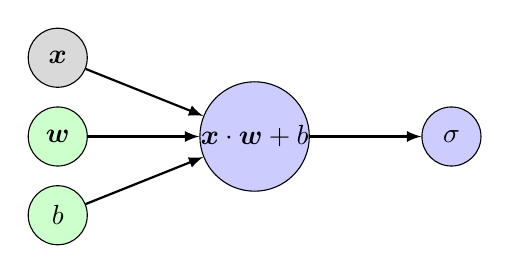
\begin{tikzpicture}	
	%\node (a1) [draw, circle, inner sep=0pt, minimum width=0.75cm, fill=green!20] {$a_1$};
	\node (x) [constant] {$\bm{x}$};
	\node (w) [param, below of=x] {$\bm{w}$};
	\node (b) [param, below of=w] {$b$};
	
	\node (f) [neuron, right of=w, xshift=1.5cm] {$\bm{x} \cdot \bm{w} + b$};
	\node (s) [neuron, right of=f, xshift=1.5cm] {$\sigma$};
	
	\begin{scope}[thick, black, ->, >=latex]
		\draw (x) -- (f);
		\draw (w) -- (f);
		\draw (b) -- (f);
		\draw (f) -- (s);
	\end{scope}	
\end{tikzpicture}
\caption{Computational graph; green circles are trainable parameters, gray are inputs}
\end{figure}
	
\end{frame}

\begin{frame}{Decision rule of log-linear model}
	
Log-linear model
$
\hat{y} = \sigma(f(\bm{x})) = \frac{1}{1 + \exp(- (\bm{x} \cdot \bm{w} + b))}
$	

\begin{itemize}
	\item Prediction = 1 if $\hat{y} > 0.5$	
	\item Prediction = 0 if $\hat{y} < 0.5$
\end{itemize}

\bigskip

Natural interpretation: Conditional probability of prediction = 1 given the input $\bm{x}$
$$
\begin{aligned}
\sigma(f(\bm{x})) &= \Pr(\text{prediction} = 1 | \bm{x}) \\
1 - \sigma(f(\bm{x})) &= \Pr(\text{prediction} = 0 | \bm{x})
\end{aligned}
$$

\end{frame}

\section{Finding the best model's parameters}

\begin{frame}{The loss function}
	
Loss function: Quantifies the loss suffered when predicting $\hat{y}$ while the true label is $y$ for a single example. In binary classification: \pause
$$
L(\hat{y}, y): \mathbb{R}^2 \to \mathbb{R}
$$

\pause
Given a labeled training set 
$(\bm{x}_{1:n}, \bm{y}_{1:n})$, 
a per-instance loss function $L$ and a
parameterized function $f(\bm{x}; \Theta)$ we define the corpus-wide loss with respect to the parameters $\Theta$ as the average loss over all training examples \pause
$$
\mathcal{L}(\Theta) = \frac{1}{n} \sum_{i =1}^{n} L (f(\bm{x}_i; \Theta), y_i)
$$
\end{frame}

\begin{frame}{Training as optimization}
$$
\mathcal{L}(\Theta) = \frac{1}{n} \sum_{i =1}^{n} L (f(\bm{x}_i; \Theta), y_i)
$$

The training examples are fixed, and the values of the parameters determine the loss

\pause
The goal of the training algorithm is to set the values of the parameters $\Theta$‚ such that
the value of $\mathcal{L}$ is minimized \pause
$$
\hat{\Theta} = \argmin_{\Theta} \mathcal{L}(\Theta) = \argmin_{\Theta} \frac{1}{n} \sum_{i =1}^{n} L (f(\bm{x}_i; \Theta), y_i)
$$


\end{frame}

\begin{frame}{Binary cross-entropy loss (logistic loss)}
$$
L_{\text{logistic}} = - y \log \hat{y} - (1 - y) \log (1 - \hat{y})
$$

\pause
\begin{block}{Partial derivative wrt.\ input $\hat{y}$}
$$
\dv{L_{\text{Logistic}}}{\hat{y}} =
- \left(
\frac{y}{\hat{y}} - \frac{1 - y}{1 - \hat{y}}
\right)
=
- \frac{y - \hat{y}}{ \hat{y} (1 - \hat{y})}
$$
\end{block}

\end{frame}

\begin{frame}{Full computational graph}
\begin{figure}
	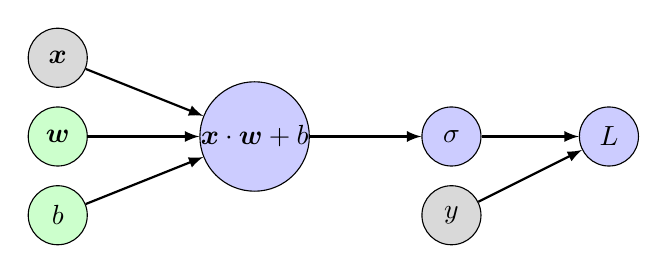
\begin{tikzpicture}	
		%\node (a1) [draw, circle, inner sep=0pt, minimum width=0.75cm, fill=green!20] {$a_1$};
		\node (x) [constant] {$\bm{x}$};
		\node (w) [param, below of=x] {$\bm{w}$};
		\node (b) [param, below of=w] {$b$};
		
		\node (f) [neuron, right of=w, xshift=1.5cm] {$\bm{x} \cdot \bm{w} + b$};
		\node (s) [neuron, right of=f, xshift=1.5cm] {$\sigma$};
		
		\node (l) [neuron, right of=s, xshift=1cm] {$L$};
		\node (y) [constant, below of=s] {$y$};
		
		\begin{scope}[thick, black, ->, >=latex]
			\draw (x) -- (f);
			\draw (w) -- (f);
			\draw (b) -- (f);
			\draw (f) -- (s);
			\draw (s) -- (l);
			\draw (y) -- (l);
		\end{scope}	
	\end{tikzpicture}
	\caption{Computational graph; green circles are trainable parameters, gray are constant inputs}
\end{figure}

How can we minimize this function?

\pause
\begin{itemize}
	\item Recall Lecture 2: (a) Gradient descent and (b) backpropagation
\end{itemize}

\end{frame}

\begin{frame}{(Online) Stochastic Gradient Descent}

\begin{algorithmic}[1]
	\Function{SGD}{$f(\bm{x}; \Theta)$, $(\bm{x}_1, \ldots, \bm{x}_n)$, $(\bm{y}_1, \ldots, \bm{y}_n)$, $L$}
	\While{stopping criteria not met}
		\State Sample a training example $\bm{x}_i, \bm{y}_i$
		\State Compute the loss $L(f(\bm{x}_i; \Theta), \bm{y}_i)$
		\State $\hat{\bm{g}} \gets$ gradient of $L(f(\bm{x}_i; \Theta), \bm{y}_i)$ wrt.\ $\Theta$
		\State $\Theta \gets \Theta - \eta_t \hat{\bm{g}}$
	\EndWhile
	\State \Return $\Theta$
	\EndFunction
\end{algorithmic}

\pause
Loss in line 4 is based on a \textbf{single training example} $\to$ a rough estimate of the corpus loss $\mathcal{L}$ we aim to minimize

\pause
The noise in the loss computation may result in inaccurate gradients

\end{frame}



\begin{frame}{Minibatch Stochastic Gradient Descent}
	
	\begin{algorithmic}[1]
		\Function{mbSGD}{$f(\bm{x}; \Theta)$, $(\bm{x}_1, \ldots, \bm{x}_n)$, $(\bm{y}_1, \ldots, \bm{y}_n)$, $L$}
		\While{stopping criteria not met}
		\State Sample $m$ examples $\{ (\bm{x}_1, \bm{y}_1), \ldots (\bm{x}_m, \bm{y}_m) \}$
		\State $\hat{\bm{g}} \gets 0$
		\For{$i = 1$ to $m$}
			\State Compute the loss $L(f(\bm{x}_i; \Theta), \bm{y}_i)$
			\State $\hat{\bm{g}} \gets \hat{\bm{g}}\ + $ gradient of $\frac{1}{m} L(f(\bm{x}_i; \Theta), \bm{y}_i)$ wrt.\ $\Theta$
		\EndFor
		\State $\Theta \gets \Theta - \eta_t \hat{\bm{g}}$
		\EndWhile
		\State \Return $\Theta$
		\EndFunction
	\end{algorithmic}
	

\end{frame}

\begin{frame}{Properties of Minibatch Stochastic Gradient Descent}

The minibatch size can vary in size from $m = 1$ to $m = n$

Higher values provide better estimates of the corpus-wide gradients, while smaller values allow more updates and in turn faster convergence

Lines 6+7: May be easily parallelized

\end{frame}


\section{Log-linear multi-class classification}

\begin{frame}{From binary to multi-class labels}
	
So far we mapped our gold label $y \in \{0, 1\}$

What if we classify into distinct categorical classes?

\begin{itemize}
	\item Categorical: There is no `ordering'
	\item Example: Classify the language of a document into 6 languages (En, Fr, De, It, Es, Other)
\end{itemize}

\pause
\begin{block}{One-hot encoding of labels}
$$
\begin{aligned}
\text{En} &= \begin{pmatrix}1 & 0 & 0 & 0 & 0 & 0\end{pmatrix} \qquad
\text{Fr} = \begin{pmatrix}0 & 1 & 0 & 0 & 0 & 0\end{pmatrix} \\
\text{De} &= \begin{pmatrix}0 & 0 & 1 & 0 & 0 & 0\end{pmatrix} \qquad \ldots \\
\bm{y} &\in \mathbb{R}^{d_{out}} \quad \text{where } d_{out} \text{ is the number of classes}
\end{aligned}
$$
\end{block}
	
\end{frame}

\begin{frame}{Possible solution: Six weight vectors and biases}
	
Consider for each language $\ell \in \{\text{En}, \text{Fr}, \text{De}, \text{It}, \text{Es}, \text{Other}\}$
\begin{itemize}
	\item Weight vector $\bm{w}^{\ell}$ (e.g., $\bm{w}^{\text{Fr}})$
	\item Bias $b^{\ell}$ (e.g., $b^{\text{Fr}})$
\end{itemize}
\pause We can predict the language resulting in the highest score
$$
\hat{y} = f(\bm{x}) = \argmax_{
\ell \in \{\text{En}, \text{Fr}, \text{De}, \text{It}, \text{Es}, \text{Other}\}
}
\bm{x} \cdot \bm{w}^{\ell} + b^{\ell}
$$

\pause
But we can re-arrange the $\bm{w} \in \mathbb{R}^{d_{in}}$ vectors into columns of a matrix $\bm{W} \in \mathbb{R}^{d_{in} \times 6}$ and $\bm{b} \in \mathbb{R}^6$, to get
$$f(\bm{x}) = \bm{x} \bm{W} + \bm{b}$$
	
\end{frame}


\begin{frame}{Projecting input vector to output vector $f(\bm{x}) : \mathbb{R}^{d_{in}} \to \mathbb{R}^{d_{out}}$}
	
\pause
\begin{block}{Recall from lecture 3: High-dimensional linear functions}
Function $f(\bm{x}) : \mathbb{R}^{d_{in}} \to \mathbb{R}^{d_{out}}$
$$f(\bm{x}) = \bm{x} \bm{W} + \bm{b}$$
where
$\bm{x} \in \mathbb{R}^{d_{in}} \qquad
\bm{W} \in \mathbb{R}^{d_{in} \times d_{out}} \qquad
\bm{b} \in \mathbb{R}^{d_{out}}$
\end{block}	
	
The simplest neural network --- a perceptron (simply a linear model)

\begin{itemize}
	\item How to find the prediction $\hat{y}$?
\end{itemize}

\end{frame}

\begin{frame}{Prediction of multi-class classifier}
Project the input $\bm{x}$ to an output $\bm{y}$
$$\bm{\hat{y}} = f(\bm{x}) = \bm{x} \bm{W} + \bm{b}$$
and pick the element of $\bm{\hat{y}}$ with the highest value
$$
\text{prediction} = \hat{y} = \argmax_{i} \bm{\hat{y}}_{[i]}
$$

\begin{block}{Sanity check}
What is $\hat{y}$?

\pause
Index of $1$ in the one-hot

For example, if $\hat{y} = 3$, then the document is in German
$\text{De} = \begin{pmatrix}0 & 0 & 1 & 0 & 0 & 0\end{pmatrix}$
\end{block}
	
\end{frame}

\subsection{Representations}


\begin{frame}{Two representations of the input document}
$$\bm{\hat{y}} = \bm{x} \bm{W} + \bm{b}$$

Vector $\bm{x}$ is a document representation
\begin{itemize}
	\item Bag of words, for example ($d_{in} = |V|$ dimensions, sparse)
\end{itemize}

Vector $\bm{\hat{y}}$ is \textbf{also} a document representation
\begin{itemize}
	\item More compact (only 6 dimensions)
	\item More specialized for the language prediction task
\end{itemize}

\end{frame}

\begin{frame}{Matrix $\bm{W}$ as learned representation --- columns}
$\bm{\hat{y}} = \bm{x} \bm{W} + \bm{b} \quad \to$ two views of $\bm{W}$, as rows or as columns

\begin{tabular}{r|cccccc}
& En & Fr & De & It & Es & Ot \\ \midrule
a & $\bullet$ & $\bullet$ & $\bullet$ & $\bullet$ & $\bullet$ & $\bullet$ \\
at & $\bullet$ & $\bullet$ & $\bullet$ & $\bullet$ & $\bullet$ & $\bullet$ \\
... & & & & & & \\
zoo & $\bullet$ & $\bullet$ & $\bullet$ & $\bullet$ & $\bullet$ & $\bullet$ \\
\end{tabular}

\pause
Each of the 6 columns (corresponding to a language) is a $d_{in}$-dimensional vector representation of this language in terms of its characteristic word unigram patterns (e.g., we can then cluster the 6 language vectors according to their similarity)


\end{frame}

\begin{frame}{Matrix $\bm{W}$ as learned representation --- rows}
$\bm{\hat{y}} = \bm{x} \bm{W} + \bm{b}$

\begin{tabular}{r|cccccc}
	& En & Fr & De & It & Es & Ot \\ \midrule
	a & $\bullet$ & $\bullet$ & $\bullet$ & $\bullet$ & $\bullet$ & $\bullet$ \\
	at & $\bullet$ & $\bullet$ & $\bullet$ & $\bullet$ & $\bullet$ & $\bullet$ \\
	... & & & & & & \\
	zoo & $\bullet$ & $\bullet$ & $\bullet$ & $\bullet$ & $\bullet$ & $\bullet$ \\
\end{tabular}

Each of the $d_{in}$ rows corresponds to a particular unigram, and provides a 6-dimensional vector
representation of that unigram in terms of the languages it prompts
	
\end{frame}

\begin{frame}{From bag-of-words to continuous bag-of-words}
\begin{block}{Recall from lecture 3 --- Averaged bag of words}
$$\bm{x} = \frac{1}{|D|} \sum_{i =1}^{|D|} \bm{x}^{D_{[i]}}$$
$D_{[i]}$ --- word in doc $D$ at position $i$, $\bm{x}^{D_{[i]}}$ --- one-hot vector
\end{block}
$$
\begin{aligned}
\bm{\hat{y}} &= \bm{x} \bm{W} = \pause
\left (\frac{1}{|D|} \sum_{i =1}^{|D|} \bm{x}^{D_{[i]}} \right) \bm{W} 
\pause = \frac{1}{|D|} \sum_{i =1}^{|D|} \left ( \bm{x}^{D_{[i]}} \bm{W} \right)  \\
&= \pause \frac{1}{|D|} \sum_{i =1}^{|D|}  \bm{W}^{D_{[i]}} 
\end{aligned}
$$
(we ignore the bias $\bm{b}$ here)
	
\end{frame}

\begin{frame}{From bag-of-words to continuous bag-of-words (CBOW)}
\begin{block}{Two equivalent views; $\bm{W}^{D_{[i]}}$ is the $D_{[i]}$-th row of matrix $\bm{W}$}
$$
\bm{\hat{y}} = \frac{1}{|D|} \sum_{i =1}^{|D|} \bm{W}^{D_{[i]}}
\qquad
\bm{\hat{y}} = \left (\frac{1}{|D|} \sum_{i =1}^{|D|} \bm{x}^{D_{[i]}} \right) \bm{W} 
$$
\end{block}

\pause
The continuous-bag-of-words (CBOW) representation
\begin{itemize}
	\item \pause Either by summing word-representation vectors
	\item \pause Or by multiplying a bag-of-words vector by a matrix in which each row corresponds to a dense word representation (also called \textbf{embedding matrix})
\end{itemize}

\end{frame}

\begin{frame}{Learned representations --- central to deep learning}
Representations are central to deep learning

One could argue that the main power of deep-learning is the ability to learn good representations
\end{frame}


\subsection{From multi-dimensional linear transformation to probabilities}

\begin{frame}{Turning output vector into probabilities of classes}

\begin{block}{Recap: Categorical probability distribution}
Categorical random variable $X$ is defined over $K$ categories, typically mapped to natural numbers $1, 2, \ldots, K$, for example En = 1, De = 2, $\ldots$

\pause
Each category parametrized with probability $\Pr(X = k) = p_k$

\pause
Must be valid probability distribution: $\sum_{i =1}^{K} \Pr(X = i) = 1$
\end{block}

\pause
How to turn an \textbf{unbounded} vector in $\mathbb{R}^K$ into a categorical probability distribution?

\end{frame}

\begin{frame}{The softmax function $\softmax (\bm{x}): \mathbb{R}^K \to \mathbb{R}^K$}

\begin{block}{Softmax}
Applied element-wise, for each element $\bm{x}_{[i]}$ we have
$$
\softmax (\bm{x}_{[i]}) = \frac{\exp(\bm{x}_{[i]})}{
	\sum_{k=1}^{K} \exp(\bm{x}_{[k]})
}
$$
\end{block}

\pause
\begin{itemize}
	\item Nominator: Non-linear bijection from $\mathbb{R}$ to $(0; \infty)$
	\item Denominator: Normalizing constant to ensure $\sum_{j = 1}^{K} \softmax (\bm{x}_{[j]}) = 1$
\end{itemize}

\pause
We also need to know how to compute the partial derivative of $\softmax (\bm{x}_{[i]})$ wrt.\ each argument $\bm{x}_{[k]}$: $\pdv{\softmax (\bm{x}_{[i]})}{\bm{x}_{[k]}}$

\end{frame}


\begin{frame}{Softmax can be smoothed with a `temperature' $T$}
\vspace{-1em}
$$
\softmax (\bm{x}_{[i]}; T) = \frac{
	\exp(\frac{\bm{x}_{[i]}}{T})
}{
	\sum_{k=1}^{K} \exp(
	\frac{\bm{x}_{[k]}}{T})
}
$$

\pause
\begin{block}{Example: Softmax of $\bm{x} = (3, 0, 1)$ at different $T$}
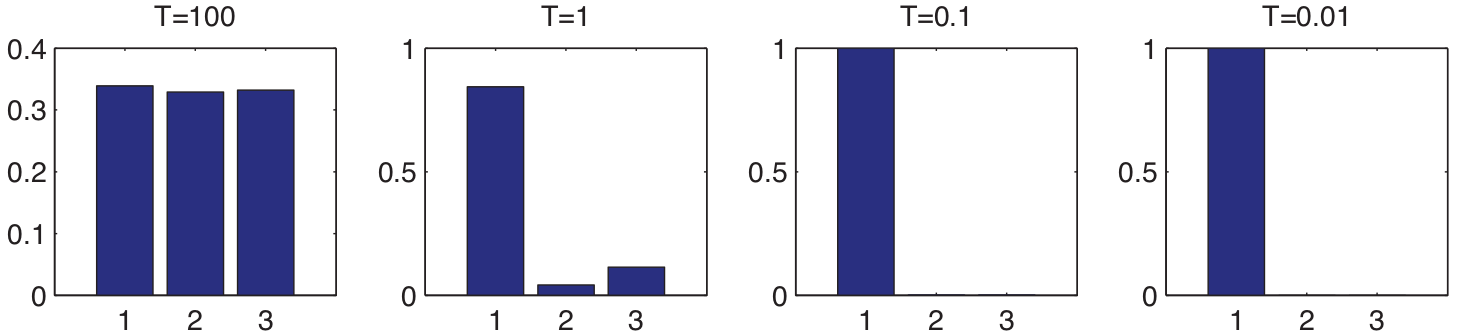
\includegraphics[width=0.95\linewidth]{img/temperatures.png}

High temperature $\to$ uniform distribution

Low temperature $\to$ `spiky' distribution, all mass on the largest element

\end{block}

\begin{tikzpicture}[overlay, remember picture] 
	\node at (current page.north east)[anchor = north east, text width=4cm, yshift=-1.3cm] {\scriptsize Figure: \fullcite[p.~103]{Murphy.2012} \par};
\end{tikzpicture}	

	
\end{frame}


\section{Loss function for softmax}

\begin{frame}{Categorical cross-entropy loss (aka.\ negative log likelihood)}

Vector representing the gold-standard categorical distribution over the classes/labels $1, \ldots, K$:
$$
\bm{y} = (\bm{y_{[1]}}, \bm{y}_{[2]}, \ldots, \bm{y}_{[K]})
$$
Output from softmax:
$$
\bm{\hat{y}} = (\bm{\hat{y}_{[1]}}, \bm{\hat{y}}_{[2]}, \ldots, \bm{\hat{y}}_{[K]})
$$
which is in fact $\bm{\hat{y}_{[i]}} = \Pr(y = i| \bm{x})$
	
	
\begin{block}{Cross entropy loss}
$$
L_{\text{cross-entropy}} (\bm{\hat{y}, \bm{y}}) =
- \sum_{k = 1}^{K} \bm{y}_{[k]} \log \left(  \bm{\hat{y}}_{[k]} \right)
$$	
\end{block}	
\end{frame}

\begin{frame}{Background: K-L divergence (also known as \emph{relative entropy})}
	
Let $Y$ and $\hat{Y}$ be categorical random variables over same categories, with probability distributions $P(Y)$ and $Q(\hat{Y})$
\begin{align*}
	\mathbb{D}(P(Y) || Q(\hat{Y})) &= \mathbb{E}_{P(Y)} \left[ \log \frac{P(Y)}{Q(\hat{Y})} \right] \\
	&= \mathbb{E}_{P(Y)} \left[ \log P(Y) - \log Q(\hat{Y}) \right] \\
	&= \mathbb{E}_{P(Y)} \left[ \log P(Y)\right] - \mathbb{E}_{P(Y)} \left[ \log Q(\hat{Y}) \right] \\
	&= - \mathbb{E}_{P(Y)} \left[ \log \frac{1}{P(Y)}\right] - \mathbb{E}_{P(Y)} \left[ \log Q(\hat{Y}) \right] \\
	&= - \mathbb{H}_{P} (Y)  - \mathbb{E}_{P(Y)} \left[ \log Q(\hat{Y}) \right] \\
\end{align*}
	
\end{frame}



\section{Stacking transformations and non-linearity}

\begin{frame}{Stacking linear layers on top of each other --- still linear!}
\vspace{-1em}
$$
\bm{x} \in \mathbb{R}^{d_{in}} \qquad
\bm{W^1} \in \mathbb{R}^{d_{in} \times d_1} \qquad
\bm{b^1} \in \mathbb{R}^{d_1} \qquad
\bm{W^2} \in \mathbb{R}^{d_1 \times d_{out}} \qquad
\bm{b^2} \in \mathbb{R}^{d_{out}} \qquad
$$
$$
f(\bm{x}) = \left(
\bm{x} \bm{W^1} + \bm{b^1}
\right)
\bm{W^2} + \bm{b^2}
$$

\begin{figure}
	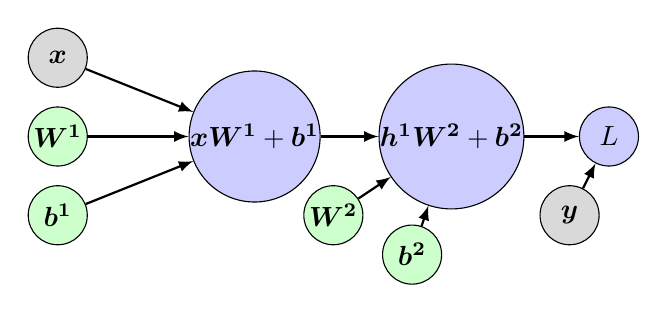
\begin{tikzpicture}	
		%\node (a1) [draw, circle, inner sep=0pt, minimum width=0.75cm, fill=green!20] {$a_1$};
		\node (x) [constant] {$\bm{x}$};
		\node (w) [param, below of=x] {$\bm{W^1}$};
		\node (b) [param, below of=w] {$\bm{b^1}$};
		
		\node (f1) [neuron, right of=w, xshift=1.5cm] {$\bm{x} \bm{W^1} + \bm{b^1}$};
		\node (f2) [neuron, right of=f1, xshift=1.5cm] {$\bm{h^1} \bm{W^2} + \bm{b^2}$};
		
		\node (w2) [param, below of=f2, xshift=-1.5cm, yshift=0cm] {$\bm{W^2}$};
		\node (b2) [param, below of=f2, xshift=-0.5cm, yshift=-0.5cm] {$\bm{b^2}$};
		
		\node (l) [neuron, right of=f2, xshift=1cm] {$L$};
		\node (y) [constant, below of=f2, xshift=1.5cm] {$\bm{y}$};
		
		\begin{scope}[thick, black, ->, >=latex]
			\draw (x) -- (f1);
			\draw (w) -- (f1);
			\draw (b) -- (f1);
			\draw (f1) -- (f2);
			\draw (f2) -- (l);
			\draw (w2) -- (f2);
			\draw (b2) -- (f2);
			\draw (y) -- (l);
		\end{scope}	
	\end{tikzpicture}
	\caption{Computational graph; green circles are trainable parameters, gray are constant inputs}
\end{figure}	
	
\end{frame}


\begin{frame}{Adding non-linear function $g: \mathbb{R}^{d_1} \to \mathbb{R}^{d_1}$}
	\vspace{-1em}
	$$
	f(\bm{x}) = g \left(
	\bm{x} \bm{W^1} + \bm{b^1}
	\right)
	\bm{W^2} + \bm{b^2}
	$$
	
	\begin{figure}
		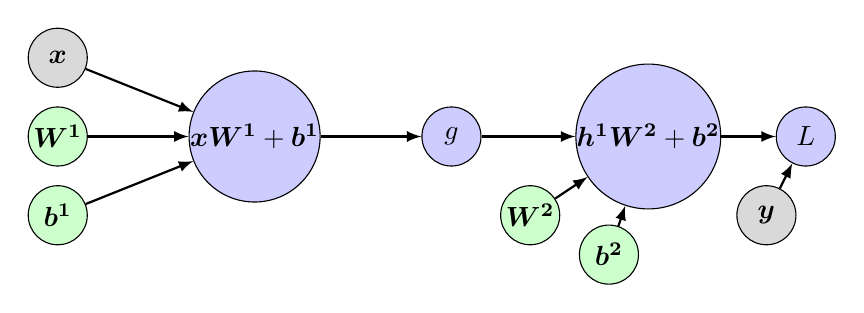
\begin{tikzpicture}	
			%\node (a1) [draw, circle, inner sep=0pt, minimum width=0.75cm, fill=green!20] {$a_1$};
			\node (x) [constant] {$\bm{x}$};
			\node (w) [param, below of=x] {$\bm{W^1}$};
			\node (b) [param, below of=w] {$\bm{b^1}$};
			
			\node (f1) [neuron, right of=w, xshift=1.5cm] {$\bm{x} \bm{W^1} + \bm{b^1}$};
			
			\node (g) [neuron, right of=f1, xshift=1.5cm] {$g$};
			\node (f2) [neuron, right of=g, xshift=1.5cm] {$\bm{h^1} \bm{W^2} + \bm{b^2}$};
			
			\node (w2) [param, below of=f2, xshift=-1.5cm, yshift=0cm] {$\bm{W^2}$};
			\node (b2) [param, below of=f2, xshift=-0.5cm, yshift=-0.5cm] {$\bm{b^2}$};
			
			\node (l) [neuron, right of=f2, xshift=1cm] {$L$};
			\node (y) [constant, below of=f2, xshift=1.5cm] {$\bm{y}$};
			
			\begin{scope}[thick, black, ->, >=latex]
				\draw (x) -- (f1);
				\draw (w) -- (f1);
				\draw (b) -- (f1);
				\draw (f1) -- (g);
				\draw (g) -- (f2);
				\draw (f2) -- (l);
				\draw (w2) -- (f2);
				\draw (b2) -- (f2);
				\draw (y) -- (l);
			\end{scope}	
		\end{tikzpicture}
		\caption{Computational graph; green circles are trainable parameters, gray are constant inputs}
	\end{figure}	
	
\end{frame}


\begin{frame}{Non-linear function $g$: Rectified linear unit (ReLU) activation}
	
	
	\begin{columns}
		
		\begin{column}{0.6\linewidth}
			
		$$
		\mathrm{ReLU}(z) =
		\begin{cases}
			0  & \quad \text{if } z < 0\\
			z  & \quad \text{if } z \geq 0
		\end{cases}
		$$
		
		or \hspace{0.4em} $\mathrm{ReLU}(z) = \max(0, x)$
		
		
			
			
		\end{column}
		
		\begin{column}{0.4\linewidth}
			\begin{figure}
				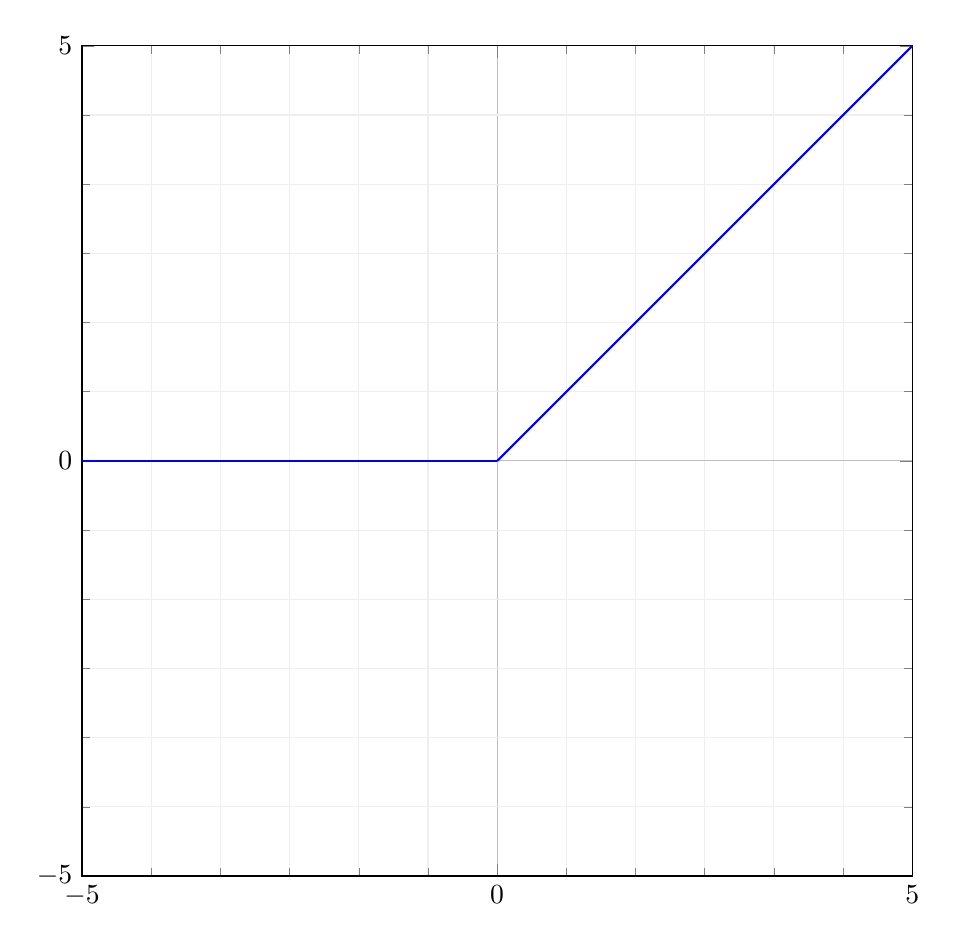
\begin{tikzpicture}
					
					\begin{axis}[
						xmin = -5, xmax = 5,
						ymin = -5, ymax = 5,
						xtick distance = 5,
						ytick distance = 5,
						grid = both,
						minor tick num = 5,
						major grid style = {lightgray},
						minor grid style = {lightgray!25},
						width = \textwidth,
						height = \textwidth,
						legend pos = north west
						]
						
						\addplot[
						domain = -5:0,
						samples = 10,
						smooth,
						thick,
						blue,
						] {0};
						
						\addplot[
						domain = 0:5,
						samples = 10,
						smooth,
						thick,
						blue,
						] {x};
						
						
					\end{axis}
					
				\end{tikzpicture}
				\caption{ReLU function}
			\end{figure}
		\end{column}
	\end{columns}
	
	
\end{frame}



\section*{Recap}

\begin{frame}{Take aways}
	
\begin{itemize}
	\item Binary classification as a linear function of words and a sigmoid
	\item Binary cross-entropy (logistic) loss
	\item Training as minimizing the loss using minibatch SGD and backpropagation
	\item Stacking layers and non-linear functions: MLP
	\item ReLU as a go-to activation function in NLP
\end{itemize}
	
\end{frame}



\begin{frame}{License and credits}

	\begin{columns}
		\begin{column}{0.7\textwidth}
			Licensed under Creative Commons Attribution-ShareAlike 4.0 International (CC BY-SA 4.0)
		\end{column}
		\begin{column}{0.2\textwidth}
			
\includegraphics[width=0.9\linewidth]{img/cc-by-sa-icon.pdf}
		\end{column}
	\end{columns}
	
	\bigskip
	
	Credits
	
	\begin{scriptsize}
		
		Ivan Habernal
		
		Content from ACL Anthology papers licensed under CC-BY \url{https://www.aclweb.org/anthology}
		
	\end{scriptsize}
	
\end{frame}



\end{document}

